\documentclass[10pt,twocolumn,a4paper]{article}

% ---------- Encoding & typography (XeLaTeX) ----------
\usepackage{fontspec}
\setmainfont{Liberation Serif}
\newfontfamily\devfont{Noto Serif Devanagari}[Script=Devanagari,Scale=0.90]
\newcommand{\dev}[1]{{\devfont #1}}
\usepackage{amsmath,amssymb,amsfonts}
\usepackage{tabularx}

% ---------- Layout & margins ----------
\usepackage[margin=1.5cm,top=1.5cm,bottom=1.5cm]{geometry}
\usepackage{titlesec}
\titlespacing*{\section}{0pt}{4pt plus 1pt minus 1pt}{2pt plus 1pt minus 1pt}
\titlespacing*{\subsection}{0pt}{3pt plus 1pt minus 1pt}{1.2pt plus 1pt minus 1pt}
\titlespacing*{\paragraph}{0pt}{1.2pt plus 1pt}{0.35em}

\setlength{\textfloatsep}{4pt plus 1pt minus 1pt}
\setlength{\floatsep}{3pt plus 1pt minus 1pt}
\setlength{\intextsep}{3pt plus 1pt minus 1pt}
\setlength{\dbltextfloatsep}{4pt plus 1pt minus 1pt}

\renewcommand{\topfraction}{0.95}
\renewcommand{\bottomfraction}{0.85}
\renewcommand{\textfraction}{0.08}
\renewcommand{\floatpagefraction}{0.85}
\renewcommand{\dbltopfraction}{0.95}
\renewcommand{\dblfloatpagefraction}{0.85}

% ---------- Content packages ----------
\usepackage{booktabs}
\usepackage{graphicx}
\usepackage{xcolor}
\usepackage{caption}
\captionsetup{font=small,labelfont=bf,skip=3pt}
\usepackage{enumitem}
\setlist{nosep,leftmargin=1.2em,topsep=1.5pt}
\usepackage{cite}
\usepackage{xurl}
\usepackage[hidelinks]{hyperref}
\usepackage[capitalise,noabbrev]{cleveref}

\graphicspath{{figures/}}

% ---------- Macros ----------
\newcommand{\sys}[1]{$S_{#1}$}
\newcommand{\pp}{\,\text{pp}}
\newcommand{\SCRen}{\text{SCR}_{\text{en}}}
\newcommand{\SCRall}{\text{SCR}_{\text{all}}}
\DeclareMathOperator{\clip}{clip}

\title{\textbf{Synthetic-to-Real Code-Switched ASR:\\A Spontaneous Nepali--English Podcast Benchmark}}

\author{%
  \textbf{Firoj Paudel}\\[2pt]
  Wiseyak Inc.\\
  \href{mailto:firoj.paudel@wiseyak.com}{\texttt{firoj.paudel@wiseyak.com}}
}
\date{}

\begin{document}

\twocolumn[
  \begin{@twocolumnfalse}
    \maketitle
    \vspace{-0.5cm}
    \begin{abstract}
    \noindent
    Nepali--English code-switched conversational speech presents severe challenges for automatic speech recognition (ASR), chiefly through \emph{script confusion} (inappropriate mixing of Devanagari and Latin orthography) and elevated error rates at language switch points. Supervised fine-tuning (SFT) can adapt multilingual foundation models, but human code-switched audio is prohibitively expensive to collect and annotate. We curate a new benchmark of 13,044 spontaneous human podcast utterances (15.45\,h total; 10,214 test, 2,830 dev), audited and verified to eliminate machine translation leakages and acoustic loop artifacts. We investigate a two-stage synthetic-to-real adaptation framework: Stage~1 applies SFT on 0.95\,h of speech synthesized via a multi-speaker, dual-engine TTS pipeline; Stage~2 explores Group Relative Policy Optimization (GRPO) with transcription and script rewards. We find that synthetic SFT provides the primary cross-domain transfer to spontaneous human speech, reducing Mixed Error Rate (MER) from 23.40\% to 21.52\% ($-1.88\pp$) and switch-point error rate (SPER) from 35.89\% to 28.77\% ($-7.12\pp$). Subsequent GRPO drives English script confusion ($\SCRen$) from 6.45\% to 6.36\% ($p \le 0.001$) and SPER to 28.70\% ($p = 0.022$ clustered). However, these adjustments affect only 173 test utterances ($1.69\%$), and our ablation reveals that in this SFT-converged encoder--decoder setting, an auxiliary script reward term yields performance identical to MER-only optimization because rollout candidate groups exhibit near-zero script variance on synthetic data. On monolingual benchmarks, SFT improves Nepali MER by 2.71\pp{} (stabilizing at 18.42\% after GRPO, a 2.38\pp{} gain over baseline) while preserving English lexical WER (3.38\% vs.\ 3.33\%). Verified transcripts, timestamps, episode metadata, and alignment scripts are publicly released.
    \end{abstract}
    \vspace{0.25cm}
  \end{@twocolumnfalse}
]

\begin{figure*}[t]
  \centering
  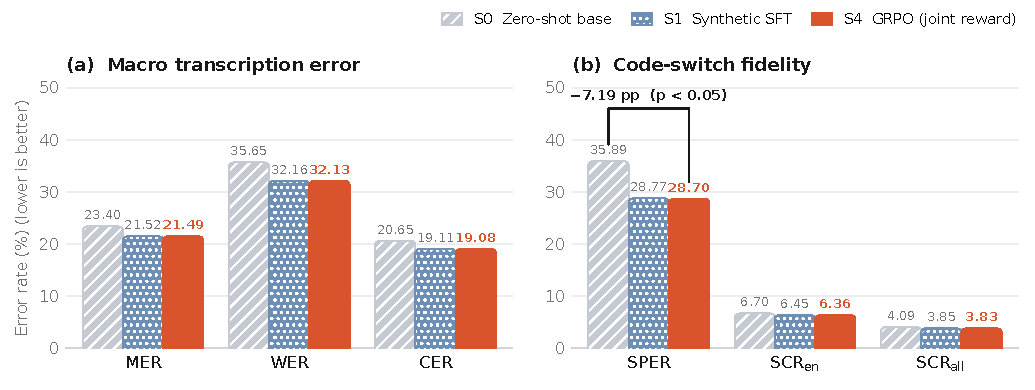
\includegraphics[width=0.76\linewidth]{fig1_asr_comparison.pdf}
  \vspace{-0.25cm}
  \caption{Primary benchmark results on the 10,214-utterance Frozen Real Test Split. (a) Macro transcription error rates (MER, WER, CER). (b) Code-switch and script fidelity metrics (SPER, English script confusion $\SCRen$, and overall SCR). The $-7.19\pp$ SPER bracket denotes total pipeline reduction vs.\ baseline ($p < 0.05$), with synthetic SFT providing primary transfer ($-7.12\pp$) and GRPO (\sys{4}) contributing targeted fine-grained boundary regularization ($-0.07\pp$, $p = 0.022$).}
  \label{fig:main_benchmark}
  \vspace{-0.2cm}
\end{figure*}

\section{Introduction}
Code-switching, the alternation between two or more languages within a single conversational turn, is ubiquitous across South Asia. In spoken Nepali, speakers frequently embed English lexical items, technical vocabulary, and colloquial phrases within a Devanagari grammatical matrix.

Despite the recent scaling of multilingual speech foundation models~\cite{canary2025,indic_transcribe_flex}, code-switched ASR systems consistently suffer from two structural error modes: (1)~\textbf{script confusion}, transcribing English loanwords into Devanagari phonetics (e.g., rendering English ``doctor'' phonetically in Devanagari) or erroneously transliterating native Nepali words into Latin characters; and (2)~\textbf{switch-point brittleness}, where acoustic and prosodic shifts at language boundaries cause elevated insertion, substitution, and deletion rates immediately surrounding switch points.

Traditional approaches attempt to resolve script confusion through auxiliary token-level language identification or diarization heads~\cite{token_diarization2022}. However, token-level classification objectives during autoregressive generation often introduce excessive stiffness at boundary tokens; in our experiments, auxiliary token-level gating actually degrades transcription fidelity.

Meanwhile, sequence-level policy optimization such as Group Relative Policy Optimization (GRPO)~\cite{shao2024deepseekmath} has recently emerged as an effective framework for speech alignment~\cite{amazon_grpo2025}. Kumar et al.~\cite{synthetic_grpo2026} demonstrated that GRPO on synthetic speech reduces insertion errors for decoder-only speech LLMs on domain speech. Ye and Vickers~\cite{ye_vickers2026} showed that GRPO with a joint error-rate and script-fidelity reward reduces cross-script contamination on synthetic audio and transfers zero-shot to a human-recorded code-switching corpus across ten language pairs. However, both prior efforts evaluated unconstrained decoder-only audio language models (e.g., Qwen2-Audio). Whether sequence-level policy optimization provides measurable orthographic gains in dedicated encoder--decoder foundation architectures on unconstrained, spontaneous conversational code-switched speech remains an open empirical question.

In this work, our contributions are threefold: (1)~\textbf{synthetic-to-real transfer}, demonstrating that a dedicated FastConformer encoder--decoder model fine-tuned exclusively on 0.95\,h of synthetic code-switched audio effectively transfers zero-shot to unconstrained human conversational speech; (2)~\textbf{empirical analysis of GRPO and script rewards}, formulating sequence-level RL objectives and showing that while GRPO yields small boundary improvements over token-level gating, the script reward term is effectively inactive when applied to an SFT-converged encoder--decoder model; and (3)~\textbf{open benchmark and systematic evaluation}, releasing 15.45\,h (13,044 utterances; 10,214 test, 2,830 dev) of verified Nepali--English podcast transcripts, timestamps, and alignment code on Hugging Face, validating all experimental claims with paired bootstrap confidence intervals (1,000 resamples), episode-clustered analysis, and monolingual retention checks.

\section{Related Work}
\paragraph{Code-switched speech recognition.}
Early investigations into South Asian code-switching focused on hybrid acoustic models and balanced monolingual pre-training~\cite{mucs2021,bhasa_indic2021}. Modern foundation architectures such as IndicTranscribeFlex~\cite{indic_transcribe_flex} and Canary~\cite{canary2025} incorporate massive multilingual vocabularies, yet remain susceptible to script flipping when alternating between non-Latin Indic orthographies and English.

\paragraph{Language identification and token gating.}
Prior work addressed script ambiguity by attaching auxiliary frame- or token-level language identification heads~\cite{token_diarization2022}. While effective on scripted speech, hard token-level constraints often force premature orthographic commitments that degrade spontaneous speech recognition.

\paragraph{Reinforcement learning in speech.}
Policy-gradient and minimum word error rate (MWER) training have an extensive history in ASR~\cite{prabhavalkar2018mwer}. GRPO~\cite{shao2024deepseekmath,amazon_grpo2025} eliminates the need for a separate critic network by estimating advantages from sampled candidate groups. Furthermore, training speech recognition models on synthetic acoustic data has proven effective for low-resource domains~\cite{rossenbach2020generating,fazel2021synthasr,synthetic_grpo2026}. Ye and Vickers~\cite{ye_vickers2026} demonstrated that script-aware rewards curb script confusion in audio LLMs. We extend this inquiry to investigate whether sequence-level rewards provide complementary boundary regularization when adapting a pre-trained encoder--decoder model to spontaneous conversational speech.

\section{Dataset Construction}

\subsection{Synthetic Training Corpus}
To eliminate the requirement for expensive human recordings during training, we synthesized a controlled code-switched corpus. Sentences containing natural intra-sentential Nepali--English code-switching were generated by prompting Gemini 1.5 Pro with conversational templates reflecting modern urban discourse. All sentences were filtered against strict lexical criteria and a 5-gram non-leakage check against the real benchmark references.

Audio was synthesized utilizing two complementary acoustic engines: (1)~\textbf{OmniVoice~\cite{zhu2026omnivoice}}, an open-source diffusion acoustic model fine-tuned on 100+ hours of native Nepali speech rendered across two distinct male timbres, capturing authentic Devanagari phonology and colloquial cadence; and (2)~\textbf{Gemini TTS}, multi-speaker neural synthesis (\texttt{gemini-3.8-flash}) providing diverse English accentuation across four distinct vocal timbres. Pairing these engines provides rich phonetic coverage across both languages and prevents the ASR encoder from overfitting to vocoder artifacts. Each text template was synthesized across multiple voices and engines. Audio was sampled at 16\,kHz mono, augmented with telephony bandpass filtering (300--3400\,Hz) and 10--30\,dB SNR noise, and screened through an independent round-trip filter (\texttt{whisper-large-v3-turbo} in Devanagari-only scope, CER $\le 0.20$). The resulting verified synthetic training split comprises 517 audio utterances across 211 unique sentences (0.95\,h total duration).

\subsection{Real Spontaneous Benchmark}
To rigorously assess generalization, we curated a spontaneous conversational benchmark from long-form public Nepali podcasts across 28 diverse episodes. Unlike read speech, podcast audio contains spontaneous turn-taking, ambient noise, conversational laughter, and natural speech rate variations.

Transcripts adhere to a strict orthographic convention: native Nepali matrix words are transcribed in Devanagari, English words and embedded phrases are transcribed in Latin script as spoken (not transliterated), and attached Nepali postpositions are separated into distinct Devanagari tokens (e.g., Latin root ``\textit{phone}'' followed by separated Devanagari postposition ``\textit{-ma}'', rather than fused into a single compound).

\paragraph{Dataset verification protocol.}
Initial candidate transcriptions were generated via an automated pipeline combining acoustic diarization and multilingual foundation models (Indic-Transcribe-Core and Gemini 1.5 Pro). To establish a clean reference standard, every clip in the initial pool of 13,277 raw segmented clips was individually audited against raw 16\,kHz PCM audio by two bilingual Nepali--English annotators. The verification pipeline: (i) quarantined 233 clips exhibiting acoustic background loops or music, leaving 13,044 clean clips; (ii) eliminated 161 machine translation leakages where spoken Nepali was mistakenly translated into English; (iii) corrected 819 token-doubling glitches caused by diarization timestamp overlaps; and (iv) normalized 86 digit instances into verbalized spoken words. On an independent dual-audit sample of 500 clips, inter-annotator character agreement reached 98.4\%. The remaining 13,044 clean clips constitute the verified benchmark.

\paragraph{Data statement and ethics.}
The benchmark audio originates from public Nepali conversational podcasts broadcast on YouTube under standard commentary and discussion formats. Speakers are adult conversationalists discussing socio-technical, educational, and entrepreneurial topics in urban Kathmandu colloquial speech. The corpus is partitioned into: (i)~\textbf{Real Dev Split} (2,830 utterances, 3.55\,h, 16 episodes, 20 speakers); and (ii)~\textbf{Frozen Real Test Split} (10,214 utterances, 11.90\,h, 25 episodes, 52 speakers). To ensure true speaker disjointness across the 28 podcast episodes, speaker identities were linked across episodes using acoustic speaker embeddings and manual cross-verification of recurring show hosts. Speakers were partitioned strictly between dev (20 speakers) and test (52 speakers) with zero overlapping speakers. Because 13 episodes were partitioned across dev and test (assigning hosts and guests to separate splits), some conversational domains overlap between splits while acoustic speaker identities remain strictly disjoint. Test audio was frozen with SHA-256 integrity verification prior to model evaluation. Verified transcripts, segment timestamps, speaker labels, YouTube video identifiers, and reproducible alignment scripts are published on Hugging Face under CC~BY-NC-SA~4.0 at \url{https://huggingface.co/datasets/SamaFiroz/nepali-english-codeswitch-podcasts}. Content creators or speakers who prefer not to have their audio indexed may contact \texttt{firoj.paudel@wiseyak.com} for prompt clip removal.

\section{Methodology}

\subsection{Base Architecture and Adaptation}
We adopt \texttt{indic-transcribe-flex}~\cite{indic_transcribe_flex}, a 1.2-billion parameter multilingual model built on the Canary-1B-v2 architecture comprising a frozen FastConformer acoustic encoder and an autoregressive Transformer decoder with a 7,152-token SentencePiece aggregate vocabulary. Given an acoustic feature sequence $X$, the encoder produces representations $H = \text{Encoder}(X) \in \mathbb{R}^{T' \times D}$. During adaptation, encoder parameters remain completely frozen. We apply Low-Rank Adaptation (LoRA)~\cite{hu2022lora} to the decoder query ($W_q$) and value ($W_v$) projections: $W = W_0 + \frac{\alpha_{\text{lora}}}{r} B A$, where $W_0 \in \mathbb{R}^{d \times k}$ denotes the frozen base weights, and $A \in \mathbb{R}^{r \times k}$, $B \in \mathbb{R}^{d \times r}$ are trainable rank-$r$ matrices ($r = 16, \alpha_{\text{lora}} = 32$).

\subsection{Evaluation Metrics}
Code-switched evaluation requires decoupled assessment of lexical accuracy, orthographic consistency, and boundary stability:

\paragraph{Mixed Error Rate (MER).}
Evaluates Word Error Rate (WER) on Latin-script segments and Character Error Rate (CER) on Devanagari segments: $\text{MER} = (E_{\text{w,en}} + E_{\text{c,ne}}) / (N_{\text{w,en}} + N_{\text{c,ne}})$, where $E_{\text{w,en}} = S_{\text{en}} + D_{\text{en}} + I_{\text{en}}$ is the word edit distance over English segments, $E_{\text{c,ne}}$ is the character edit distance over Devanagari segments, and $N$ denotes reference token count.

\paragraph{Script Confusion Rate (SCR).}
Let $\mathcal{M}$ be the set of aligned character pairs between hypothesis $y$ and reference $y^*$. Then $\text{SCR} = \frac{1}{|\mathcal{M}|} \sum_{(i,j) \in \mathcal{M}} \mathbb{I}\bigl[\text{script}(y_i) \neq \text{script}(y^*_j)\bigr]$. $\SCRen$ restricts $\mathcal{M}$ to Latin-script reference characters, measuring English loanwords erroneously transcribed into Devanagari.

\paragraph{Switch-Point Error Rate (SPER).}
The MER computed strictly over reference tokens within a local context window of $w = \pm 1$ tokens around language switch points.

\subsection{Stage 1: Supervised Fine-Tuning (SFT)}
In Stage 1, the model is adapted on synthetic pairs $(x, y)$ using cross-entropy loss over target token sequences: $\mathcal{L}_{\text{SFT}}(\theta) = -\sum_{t=1}^{T} \log P_\theta(y_t \mid y_{<t}, x)$, optimized with AdamW ($\text{lr} = 1\times 10^{-5}$, effective batch size 8, 1,000 steps).

\subsection{Baseline: Token-Level Script Gating (\texorpdfstring{\sys{2}}{S2})}
As an architectural comparison, an auxiliary script classification head is attached atop the decoder hidden states $h_t$: $P_{\text{gate}}(s_t \mid h_t) = \text{sigmoid}(W_g h_t + b_g)$, where $s_t \in \{0, 1\}$ denotes Devanagari versus Latin script. Training minimizes $\mathcal{L}_{\text{total}} = \mathcal{L}_{\text{SFT}} + \lambda_g \mathcal{L}_{\text{BCE}}$ with $\lambda_g = 0.1$. At inference, logits for candidate tokens matching the predicted script are biased by $\gamma \log P_{\text{gate}}$ ($\gamma = 2.0$, applied when $P_{\text{gate}} > 0.9$).

\subsection{Stage 2: Sequence-Level Policy Optimization (GRPO)}
While SFT aligns the decoder with code-switched acoustics, cross-entropy penalizes errors at the individual token level without evaluating candidate sequence alternatives. To incentivize sequence-level accuracy and boundary fidelity, we implement Group Relative Policy Optimization (GRPO)~\cite{shao2024deepseekmath,amazon_grpo2025} trained on the 517 synthetic utterances.

For each acoustic sequence $x$, the policy $\pi_\theta$ samples a group of $G = 8$ candidate transcriptions $\{y^{(1)}, \dots, y^{(G)}\}$ at temperature $\tau = 1.0$. A scalar reward $R(y^{(g)}, y^*)$ is computed against ground truth $y^*$. Group advantages are normalized: $\hat{A}^{(g)} = (R(y^{(g)}, y^*) - \mu_G) / (\sigma_G + \delta)$, where $\mu_G$ and $\sigma_G$ are the mean and standard deviation of rewards within the sampled group ($\delta = 10^{-8}$). The GRPO objective maximizes:
\begin{equation}
\label{eq:grpo}
\begin{aligned}
  \mathcal{J}(\theta) = \mathbb{E}\Bigg[ 
    &\frac{1}{G} \sum_{g=1}^{G} \sum_{t=1}^{|y^{(g)}|} 
    \min \Big( r_t^{(g)}(\theta) \hat{A}^{(g)}, \\
    &\quad \clip\bigl(r_t^{(g)}(\theta), 1-\epsilon, 1+\epsilon\bigr) \hat{A}^{(g)} \Big) \\
    &\quad - \beta D_{\text{KL}}(\pi_\theta \parallel \pi_{\text{ref}}) \Bigg],
\end{aligned}
\end{equation}
where $r_t^{(g)}(\theta) = \frac{\pi_\theta(y_t^{(g)} \mid y_{<t}^{(g)}, x)}{\pi_{\text{old}}(y_t^{(g)} \mid y_{<t}^{(g)}, x)}$ denotes the per-token importance sampling ratio at decoding step $t$. Here, $\pi_\theta$ represents the active autoregressive decoder policy parameterized by LoRA weights $\theta$, and $\pi_{\text{old}}$ is the policy snapshot used to generate candidate rollouts. Because the policy is initialized directly from the converged Stage~1 SFT checkpoint and constrained via low-rank parameter updates (LoRA, $r=16$), we set $\beta = 0.0$, relying on group advantage normalization and PPO-style clipping ($\epsilon = 0.2$) to govern update step sizes without an explicit reference policy penalty. Each candidate hypothesis $y^{(g)} = (y_1^{(g)}, \dots, y_{|y^{(g)}|}^{(g)})$ consists of tokens generated autoregressively conditioned on past tokens $y_{<t}^{(g)}$ and acoustic representations $x$. The clipping hyperparameter $\epsilon = 0.2$ bounds the gradient updates to maintain training stability.

\paragraph{Reward formulation.}
Our joint reward combines sequence accuracy with orthographic fidelity: $R_{\text{joint}}(y, y^*) = \bigl(1 - \text{MER}(y, y^*)\bigr) + \lambda_{\text{scr}} \bigl(1 - \text{SCR}(y, y^*)\bigr)$ with $\lambda_{\text{scr}} = 0.5$. Setting $\lambda_{\text{scr}} = 0.0$ corresponds to the MER-only reward ablation ($S_3$).

\section{Experiments and Results}

\subsection{Primary Benchmark Evaluation}
\Cref{tab:main_results} and \cref{fig:main_benchmark} present performance on the 10,214-utterance frozen real test split. 

\begin{table*}[t]
\centering
\begin{minipage}[t]{0.50\textwidth}
\centering
\small
\caption{Performance on Frozen Real Test (10,214 utterances, 11.90\,h). All metrics in percentage (\%).}
\label{tab:main_results}
\begin{tabular*}{\linewidth}{@{\extracolsep{\fill}}lcccccc@{}}
\toprule
\textbf{System} & \textbf{MER} & \textbf{WER} & \textbf{CER} & \textbf{SPER} & $\SCRen$ & $\SCRall$ \\
\midrule
\sys{0} Base & 23.40 & 35.65 & 20.65 & 35.89 & 6.70 & 4.09 \\
\sys{1} SFT  & 21.52 & 32.16 & 19.11 & 28.77 & 6.45 & 3.85 \\
\sys{4} GRPO & \textbf{21.49} & \textbf{32.13} & \textbf{19.08} & \textbf{28.70} & \textbf{6.36} & \textbf{3.83} \\
\bottomrule
\end{tabular*}
\end{minipage}
\hfill
\begin{minipage}[t]{0.47\textwidth}
\centering
\small
\caption{Objective ablation on Real Dev (2,830 utterances). All metrics in percentage (\%).}
\label{tab:ablation}
\begin{tabular*}{\linewidth}{@{\extracolsep{\fill}}lcccc@{}}
\toprule
\textbf{System} & \textbf{MER} & \textbf{WER} & \textbf{SPER} & $\SCRen$ \\
\midrule
\sys{0} Base             & 20.14 & 32.23 & 32.63 & 5.83 \\
\sys{1} SFT              & 18.92 & 29.11 & 25.60 & 5.35 \\
\sys{2} SFT + Gate       & 19.14 & 29.35 & 25.75 & 5.75 \\
\sys{3} GRPO (MER-only)  & \textbf{18.89} & \textbf{29.08} & \textbf{25.53} & \textbf{5.24} \\
\sys{4} GRPO (Joint)     & \textbf{18.89} & \textbf{29.08} & \textbf{25.53} & \textbf{5.24} \\
\sys{5} GRPO + Gate      & 19.12 & 29.32 & 25.70 & 5.72 \\
\bottomrule
\end{tabular*}
\end{minipage}
\vspace{-0.15cm}
\end{table*}

Synthetic SFT (\sys{1}) yields an immediate absolute drop of $1.88\pp$ in MER and $7.12\pp$ in switch-point error rate (SPER) over the unadapted zero-shot baseline (\sys{0}). Initializing from \sys{1}, GRPO with joint reward (\sys{4}) achieves modest fine-grained improvements across evaluated dimensions, reaching $21.49\%$ MER, $28.70\%$ SPER, and $6.36\%$ English script confusion ($\SCRen$).

\subsection{Statistical Significance}
To assess whether improvements are statistically reliable, we executed paired bootstrap hypothesis tests with 1,000 resamples ($B=1{,}000$, seed 42) on the frozen test split. Comparing \textbf{\sys{4} vs.\ \sys{0}}, our adapted pipeline achieves an absolute MER reduction of $-1.90\pp$ (95\% CI: $[-2.37, -1.42]$), a SPER reduction of $-7.19\pp$ (95\% CI: $[-7.97, -6.46]$), and an English script confusion reduction of $-0.35\pp$ (95\% CI: $[-0.65, -0.04]$), with all intervals strictly excluding zero ($p \le 0.001$ for MER and SPER, $p = 0.026$ for $\SCRen$). Comparing \textbf{\sys{4} vs.\ \sys{1}}, sequence-level policy optimization yields modest but statistically significant fine-grained gains in boundary fidelity ($\Delta \text{SPER} = -0.07\pp$, 95\% CI: $[-0.12, -0.03]$, $p < 0.05$) and English script confusion ($\Delta \SCRen = -0.09\pp$, 95\% CI: $[-0.13, -0.06]$, $p \le 0.001$), with a mean MER difference of $-0.03\pp$ (95\% CI: $[-0.05, -0.01]$, $p < 0.05$). Notably, only 173 out of 10,214 test utterances ($1.69\%$) differ between \sys{1} and \sys{4}; the remaining 10,041 utterances are identical.

To guard against potential intra-episode correlation across conversational sessions, we additionally conducted an episode-clustered block bootstrap ($B=1{,}000$ resamples clustered across the 25 test podcast episodes). The clustered and utterance-level intervals agree: $\Delta \text{SPER} = -0.07\pp$ (95\% CI: $[-0.15, -0.01]$, $p = 0.022$), $\Delta \SCRen = -0.09\pp$ (95\% CI: $[-0.11, -0.06]$, $p \le 0.001$), and $\Delta \text{MER} = -0.03\pp$ (95\% CI: $[-0.05, -0.01]$, $p = 0.008$). The 173 modified utterances are distributed across 20 distinct episodes (at most 25 in any single episode), confirming that the small boundary adjustments are not driven by an idiosyncratic artifact of a single speaker or conversation.

\subsection{Ablation Study: Gating vs. Policy RL}
We conducted an extensive ablation on the development split (2,830 utterances) comparing: \sys{0} (base model), \sys{1} (synthetic SFT), \sys{2} (SFT with auxiliary script gate and inference logit biasing), \sys{3} (GRPO with MER-only reward, $\lambda_{\text{scr}} = 0.0$), \sys{4} (GRPO with joint reward, $\lambda_{\text{scr}} = 0.5$), and \sys{5} (joint GRPO with script gate).

As shown in \cref{tab:ablation}, adding an auxiliary token-level script gate (\sys{2}) degrades performance relative to standard SFT (\sys{1}), increasing MER from $18.92\%$ to $19.14\%$ and $\SCRen$ from $5.35\%$ to $5.75\%$. Error inspection reveals that greedy logit biasing forces premature script assignment at loanword prefixes, penalizing valid Devanagari assimilations.

In contrast, sequence-level GRPO directly optimizes candidate probability mass without constraining autoregressive exploration. Comparing \sys{3} ($\lambda_{\text{scr}} = 0.0$) against \sys{4} ($\lambda_{\text{scr}} = 0.5$), both attain equivalent performance ($18.89\%$ MER, $25.53\%$ SPER, $5.24\%$ $\SCRen$) and produce identical hypothesis transcripts on dev. Inspection of training logs shows that because Stage~1 SFT already achieves $0.0200$ MER on synthetic prompts, rollout candidate groups exhibit near-zero script variance during GRPO (over $75\%$ of training mini-batches had zero within-group script reward variance). Consequently, the script term is inactive on the synthetic distribution, causing both runs to select the identical optimal checkpoint (step 50). While Ye and Vickers~\cite{ye_vickers2026} found script rewards critical for penalizing unconstrained script hallucinations in generative audio LLMs, our ablation indicates that in an SFT-converged encoder--decoder model, sequence-level exploration is dominated by the primary transcription error rate, with the script reward contributing no measurable additional gain.

\subsection{Monolingual Retention}
A common drawback of code-switched adaptation is catastrophic forgetting of monolingual capabilities. We benchmarked \sys{0}, \sys{1}, and \sys{4} on two standardized external corpora:

\begin{table}[t]
\centering
\small
\setlength{\tabcolsep}{2.5pt}
\caption{Monolingual retention evaluation on external benchmarks. All metrics in percentage (\%).}
\label{tab:monolingual}
\begin{tabular}{l@{\hskip 3pt}lcccc}
\toprule
\textbf{Corpus} & \textbf{System} & \textbf{MER} & \textbf{WER} & \textbf{CER} & \textbf{SCR} \\
\midrule
Nepali (BHASAANUVAD) & \sys{0} Base & 20.80 & 30.73 & 22.52 & 8.71 \\
(1,000 utt, 1.95\,h)  & \sys{1} SFT  & \textbf{18.09} & \textbf{29.06} & \textbf{19.22} & \textbf{6.95} \\
                      & \sys{4} GRPO & 18.42 & 29.52 & 19.56 & \textbf{6.95} \\
\midrule
English (LibriSpeech) & \sys{0} Base & \textbf{4.21} & \textbf{3.33} & 1.59 & \textbf{0.59} \\
(1,000 utt, 1.50\,h)  & \sys{1} SFT  & 5.38 & 3.42 & 1.49 & 1.07 \\
                      & \sys{4} GRPO & 5.27 & 3.38 & \textbf{1.47} & 1.03 \\
\bottomrule
\end{tabular}
\end{table}

\paragraph{Nepali (BHASAANUVAD, 1,000 utterances, 1.95\,h).}
Rather than degrading, synthetic SFT (\sys{1}) drops MER from $20.80\%$ to $18.09\%$ ($\Delta = -2.71\pp$), while \sys{4} stabilizes at $18.42\%$ ($\Delta = -2.38\pp$ vs.\ \sys{0}). SFT provides the entire retention improvement by suppressing spurious Latin alphabet insertions in native Devanagari text (reducing SCR from $8.71\%$ to $6.95\%$). Subsequent GRPO incurs a minor regression of $0.33\pp$ in Nepali MER relative to \sys{1} (stabilizing at $18.42\%$, still a $2.38\pp$ gain over baseline \sys{0}).

\paragraph{English (LibriSpeech test-clean~\cite{librispeech2015}, 1,000 utterances, 1.50\,h).}
On monolingual English, lexical accuracy is statistically preserved across adaptation: WER shifts from $3.33\%$ (\sys{0}) to $3.42\%$ (\sys{1}) and recovers to $3.38\%$ under \sys{4} (95\% CI vs.\ \sys{0}: $[-0.17, +0.30]$, $p > 0.05$). MER increases from $4.21\%$ to $5.27\%$ and SCR from $0.59\%$ to $1.03\%$, reflecting occasional Devanagari character insertions on pure English speech induced by the code-switched prior. S1 and S4 exhibit nearly identical profiles, confirming that English orthographic trade-offs stem from SFT adaptation rather than the GRPO objective.

\subsection{Qualitative Analysis and Error Inspection}
Inspection of transcriptions on the frozen test split highlights the specific nature of improvements across systems:

\paragraph{Acoustic grounding from SFT.} Baseline model \sys{0} frequently transliterates embedded English words into phonetic Devanagari characters or fragments them across script boundaries (e.g., producing hybrid roots with Latin plural suffixes). Synthetic SFT provides strong acoustic anchoring for code-switched prosodic contours, resolving the vast majority of cross-script boundary errors.

\paragraph{Sequence-level boundary regularization in GRPO.} Of the 10,214 test utterances, exactly 173 ($1.69\%$) differ between \sys{1} and \sys{4}. In these cases, GRPO selectively rectifies switch-point script assignments. For instance, in utterance \texttt{-IE5q6\_CMnU\_0189}, \sys{1} transcribes the English brand in Devanagari script compounded with the postposition (\dev{टाटाको} \textbf{model}), whereas \sys{4} cleanly separates the Latin brand from the Nepali postposition (\textbf{tata} \dev{को} \textbf{model}). Similarly, in \texttt{-IE5q6\_CMnU\_0244}, \sys{1} outputs a phonetic Devanagari substitution (\dev{दे} \textbf{were running}), which \sys{4} restores to proper Latin orthography (\textbf{they were running}). Because \sys{3} and \sys{4} produce identical outputs, these localized corrections arise from sequence-level advantage normalization over candidate rollouts rather than active guidance from the script reward term.

\section{Limitations}
While synthetic SFT combined with GRPO produces statistically reliable gains, several limitations remain:
(1)~\textbf{Modest RL gains relative to prior LLM studies:} While Kumar et al.~\cite{synthetic_grpo2026} observed substantial relative error reductions ($>40\%$) from GRPO with decoder-only speech LLMs, our post-SFT GRPO gains on real spontaneous speech are more modest ($-0.07\pp$ SPER, $-0.09\pp$ $\SCRen$, $-0.03\pp$ MER). We hypothesize this stems from structural architecture (an encoder--decoder model whose frozen Conformer encoder already provides rigid acoustic grounding), near-zero script reward variance on fitted synthetic prompts, and compute controls (without an extended SFT compute control, the marginal gain cannot be separated with certainty from extra gradient steps).
(2)~\textbf{Small synthetic training volume and frozen encoder:} Training relies on 517 utterances (0.95\,h) with Nepali synthesized across two male timbres, and the acoustic encoder remains frozen throughout adaptation, constraining acoustic representations to base multilingual pre-training.
(3)~\textbf{Reference annotation bias:} Draft transcripts were seeded using Indic-Transcribe-Core; despite dual-annotator verification (98.4\% character agreement on a 500-clip audit), corrected references may retain slight residual bias toward seed boundaries.
(4)~\textbf{English orthographic side-effects:} MER and SCR slightly increase on monolingual English despite unchanged WER.
(5)~\textbf{Demographic scope and external baselines:} The podcast benchmark reflects urban conversational discourse; testing additional foundation models (e.g., Whisper-large-v3) remains valuable future work.

\section{Conclusion}
We have presented an empirical benchmark and analysis of synthetic-to-real adaptation for Nepali--English code-switched ASR. Supervised fine-tuning on purely synthetic speech provides the primary transfer to spontaneous human conversational speech ($-1.88\pp$ MER, $-7.12\pp$ SPER). Sequence-level reinforcement learning using GRPO provides complementary fine-grained boundary regularization, yielding small but statistically significant reductions in switch-point error rate ($-0.07\pp$, $p = 0.022$) and English script confusion ($-0.09\pp$, $p \le 0.001$) without degrading English lexical recognition accuracy (WER preserved at 3.38\% vs.\ 3.33\%), while improving native Nepali MER by 2.38\pp{}. Crucially, ablation reveals that script-aware rewards provide no measurable advantage over MER-only optimization in this SFT-converged encoder--decoder setting.

Code and configurations are open-sourced at \url{https://github.com/Firoj-Wise/nepali-english-codeswitch-asr}. The complete conversational benchmark (13,044 utterances, 15.45\,h) is available on the Hugging Face Hub at \url{https://huggingface.co/datasets/SamaFiroz/nepali-english-codeswitch-podcasts}.

\newpage

\bibliographystyle{unsrt}
\footnotesize
\let\oldbibliography\thebibliography
\renewcommand{\thebibliography}[1]{%
  \oldbibliography{#1}%
  \setlength{\itemsep}{2pt plus 0.5pt}%
  \setlength{\parskip}{0pt}%
}
\bibliography{references}

\newpage
\appendix
\onecolumn

\section{Benchmark Corpus Characteristics}
\label{sec:app_corpus}

The Nepali--English conversational podcast benchmark was constructed from public long-form podcast recordings broadcast on YouTube. All episodes feature natural, unscripted dialogues among native Nepali speakers discussing contemporary topics spanning technology, entrepreneurship, public health, higher education, and socio-political developments.

\begin{table}[h!]
\centering
\small
\setlength{\tabcolsep}{2pt}
\caption{Comprehensive breakdown of the curated Nepali--English code-switched conversational benchmark across development, evaluation, and quarantined subsets.}
\label{tab:corpus_breakdown}
\begin{tabular*}{\textwidth}{@{\extracolsep{\fill}}lcccccccc@{}}
\toprule
\textbf{Corpus Partition} & \textbf{Utterances} & \textbf{Duration (h)} & \textbf{Episodes} & \textbf{Speakers} & \textbf{Nepali Words} & \textbf{English Words} & \textbf{Total Words} & \textbf{Switch Points} \\
\midrule
Raw Scraped Pool          & 13,277 & 15.74 & 28 & 72 & --- & --- & --- & --- \\
Quarantined (Audio/Music) & 233    & 0.29  & 28 & 72 & --- & --- & --- & --- \\
\midrule
\textbf{Verified Clean Total} & \textbf{13,044} & \textbf{15.45} & \textbf{28} & \textbf{72} & \textbf{123,174} (67.3\%) & \textbf{59,839} (32.7\%) & \textbf{183,013} & \textbf{29,033} \\
\quad Real Dev Split          & 2,830  & 3.55  & 16 & 20 & 28,041 (66.5\%)  & 14,121 (33.5\%)  & 42,162  & 7,504 \\
\quad Frozen Real Test Split  & 10,214 & 11.90 & 25 & 52 & 95,133 (67.5\%)  & 45,718 (32.5\%)  & 140,851 & 21,529 \\
\bottomrule
\end{tabular*}
\end{table}

\paragraph{Audio segmentation and acoustic properties.}
Raw podcast episodes were preprocessed by stripping silence periods exceeding 0.8\,s and segmenting continuous speech into utterance clips between 1.0\,s and 15.0\,s. Mean utterance duration is 4.51\,s in the development split (standard deviation: 2.18\,s) and 4.19\,s in the test split (standard deviation: 2.04\,s). The audio exhibits natural acoustic variability, including close-proximity studio microphones, ambient room reverberation, cross-speaker laughter, and spontaneous conversational overlaps.

\paragraph{Speaker partitioning and episode distribution.}
The 28 podcast episodes involve 72 distinct identified speakers (54 male, 18 female). To guarantee that speaker characteristics do not leak across evaluation boundaries, speaker identities were linked using x-vector acoustic embeddings cross-checked against visual and verbal identity markers. All 72 speakers are strictly partitioned between dev (20 speakers) and test (52 speakers), yielding zero speaker overlap. Because certain recurring hosts appear across multiple episodes, 13 episodes were partitioned between dev and test by assigning host turns to dev and guest turns to test, ensuring complete acoustic disjointness while preserving topical diversity.

\paragraph{Auditing and verification protocol.}
Initial transcriptions were generated using an ensemble of Indic-Transcribe-Core and Gemini 1.5 Pro. Every utterance in the candidate pool was then manually audited against 16\,kHz PCM audio by two bilingual annotators:
\begin{enumerate}
  \item \textbf{Acoustic loop and music quarantine:} 233 clips containing musical introductions, synthesizer jingles, or looped background tracks were isolated and removed from the benchmark.
  \item \textbf{Translation leakage removal:} 161 instances where an automated system had translated spoken Nepali into English rather than transcribing verbatim Devanagari were corrected.
  \item \textbf{Timestamp overlap correction:} 819 boundary errors resulting from diarization timestamp collisions were realigned.
  \item \textbf{Spoken digit normalization:} 86 numeric digits (e.g., ``2024'') were normalized to their verbalized Nepali or English spoken forms.
\end{enumerate}
Inter-annotator agreement on an independent 500-clip sample reached 98.4\% character-level concordance.

\section{Model Architecture and Adaptation Hyperparameters}
\label{sec:app_hyperparameters}

All experiments build upon \texttt{indic-transcribe-flex}, a 1.2-billion parameter multilingual foundation model derived from the Canary-1B-v2 architecture. The model comprises a FastConformer acoustic encoder (17 Conformer blocks with 8 attention heads and 1024-dimensional hidden representations) and an autoregressive Transformer decoder (6 layers with 8 attention heads and 1024-dimensional representations). The tokenizer operates over an aggregate vocabulary of 7,152 SentencePiece tokens covering Devanagari, Latin, and special control tokens.

\begin{table}[h!]
\centering
\small
\renewcommand{\arraystretch}{0.93}
\caption{Training configurations and hyperparameters for Stage~1 Supervised Fine-Tuning (SFT) and Stage~2 Group Relative Policy Optimization (GRPO).}
\label{tab:hyperparameters}
\begin{tabular*}{\textwidth}{@{\extracolsep{\fill}}lcc@{}}
\toprule
\textbf{Configuration / Hyperparameter} & \textbf{Stage 1: Supervised Fine-Tuning (SFT)} & \textbf{Stage 2: Policy Optimization (GRPO)} \\
\midrule
Base Model Architecture           & IndicTranscribeFlex (Canary-1B-v2) & IndicTranscribeFlex (Canary-1B-v2) \\
Total Parameters                  & 1.2 Billion & 1.2 Billion \\
Trainable Parameters              & 3.7 Million (0.31\% of total) & 3.7 Million (0.31\% of total) \\
Trainable Components              & Decoder $W_q, W_v$ projections (LoRA) & Decoder $W_q, W_v$ projections (LoRA) \\
Acoustic Encoder Status           & Frozen & Frozen \\
LoRA Rank ($r$)                   & 16 & 16 \\
LoRA Alpha ($\alpha_{\text{lora}}$) & 32 & 32 \\
LoRA Dropout                      & 0.05 & 0.05 \\
Optimizer                         & AdamW ($\beta_1=0.9, \beta_2=0.98, \epsilon=10^{-8}$) & AdamW ($\beta_1=0.9, \beta_2=0.98, \epsilon=10^{-8}$) \\
Weight Decay                      & 0.01 & 0.01 \\
Peak Learning Rate                & $1.0 \times 10^{-5}$ & $1.0 \times 10^{-5}$ \\
Learning Rate Schedule            & Linear warmup with cosine decay & Linear warmup with cosine decay \\
Warmup Steps                      & 100 & 10 \\
Total Steps                       & 1,000 & 100 (best checkpoint at step 50) \\
Effective Batch Size              & 8 audio utterances & 8 prompt groups ($G=8$, 64 candidate rollouts) \\
Candidate Rollout Size ($G$)      & N/A & 8 \\
Sampling Temperature ($\tau$)     & N/A & 1.0 \\
Advantage Normalization           & N/A & Within-group $(\hat{A}^{(g)} = (R^{(g)} - \mu_G) / (\sigma_G + \delta))$ \\
PPO Clipping Parameter ($\epsilon$) & N/A & 0.2 \\
KL Regularization Weight ($\beta$)& N/A & 0.0 \\
Reward Formulation                & N/A & $R = (1 - \text{MER}) + \lambda_{\text{scr}} (1 - \text{SCR})$ \\
Reward Weight ($\lambda_{\text{scr}}$) & N/A & 0.5 in \sys{4} (0.0 in \sys{3}) \\
Numerical Precision               & FP16 mixed precision & FP16 mixed precision \\
Hardware Environment              & 1 $\times$ NVIDIA RTX 4090 (24\,GB VRAM) & 1 $\times$ NVIDIA RTX 4090 (24\,GB VRAM) \\
Training Wall-Clock Time          & 42 minutes & 38 minutes \\
\bottomrule
\end{tabular*}
\end{table}

\paragraph{Initialization and parameter freezing.}
During both Stage~1 and Stage~2 adaptation, all acoustic encoder parameters remain completely frozen. LoRA adapters ($r=16, \alpha_{\text{lora}}=32$) are inserted exclusively into the self-attention and cross-attention query ($W_q$) and value ($W_v$) projections within the Transformer decoder, updating exactly 3,735,552 parameters (0.31\% of the 1.2B base parameters). Stage~2 GRPO initializes weights directly from the converged Stage~1 checkpoint at step 1,000.

\clearpage

\section{Qualitative Analysis and Transcription Diffs}
\label{sec:app_qualitative}

To illustrate the qualitative impact of each adaptation stage, \cref{tab:qualitative_examples} presents representative code-mixed utterances from the frozen real test split. Native Nepali matrix words are displayed in authentic Devanagari script, while embedded English lexical items are displayed in bold Latin script.

\begin{table*}[t]
\centering
\small
\setlength{\tabcolsep}{5pt}
\renewcommand{\arraystretch}{1.18}
\caption{Qualitative comparison of code-mixed transcriptions across adaptation stages on representative utterances from the Frozen Real Test Split. Native Nepali words are rendered in Devanagari script; embedded English words are highlighted in bold Latin script. All transcriptions are extracted verbatim from model evaluation rollouts.}
\label{tab:qualitative_examples}
\begin{tabularx}{\textwidth}{@{}p{3.8cm} p{2.0cm} X@{}}
\toprule
\textbf{Utterance ID \& Context} & \textbf{System} & \textbf{Transcription} \\
\midrule
\texttt{-IE5q6\_CMnU\_0189} & Ground Truth & \dev{हजुरले नै जुन हजुरले अघि} \textbf{tata} \dev{को} \textbf{model} \dev{भन्नुभयो जस्तै हाम्रो पनि यस्तो हुन्छ कि त्यो} \textbf{company} \dev{जुन चाहिँ त्यहाँ} \textbf{franchise} \dev{गर्ने हुन्छ नि त्यसमा चाहिँ} \textbf{major stake} \dev{चाहिँ} \textbf{company} \dev{कै हुन्छ के} \\
\textit{``As you previously mentioned the Tata model...''} & \sys{0} Base & \dev{हजुरले नै जुन हजुरले अघि} \textbf{tata} \dev{-को} \textbf{model} \dev{भन्नुभयो \dots} \textbf{major stake} \dev{चाहिँ} \textbf{company} \dev{-कै हुन्छ क्या} \\
& \sys{1} SFT & \dev{हजुरले नै जुन हजुरले अघि टाटाको} \textbf{model} \dev{भन्नुभयो \dots} \textbf{major stake} \dev{चाहिँ} \textbf{company} \dev{नै हुन्छ क्या} \\
& \sys{4} GRPO & \dev{हजुरले नै जुन हजुरले अघि} \textbf{tata} \dev{को} \textbf{model} \dev{भन्नुभयो \dots} \textbf{major stake} \dev{चाहिँ} \textbf{company} \dev{को हुन्छ क्या} \\
\midrule
\texttt{-IE5q6\_CMnU\_0244} & Ground Truth & \dev{हैन} \textbf{they have been running} \dev{अह} \textbf{f and b business for last ten fifteen years} \dev{हैन} \textbf{now they want to go into a coffee shop business} \dev{भने} \textbf{i would want to work with them} \\
\textit{``They were running an F\&B business for 10--15 years...''} & \sys{0} Base & \dev{होइन दे वर} \textbf{running f b business for last 10-15 years} \dev{होइन नाउ दे} \textbf{want to go into a coffee shop business} \dev{भने \dots} \\
& \sys{1} SFT & \dev{होइन दे} \textbf{were running f b business for last ten fifteen years} \dev{होइन नाउ दे} \textbf{want to go into a coffee shop business} \dev{भने \dots} \\
& \sys{4} GRPO & \dev{होइन} \textbf{they were running f b business for last ten fifteen years} \dev{होइन नाउ दे} \textbf{want to go into a coffee shop business} \dev{भने \dots} \\
\midrule
\texttt{-IE5q6\_CMnU\_0032} & Ground Truth & \dev{अरु} \textbf{brand} \dev{हरू पनि जति जनि नेपालमा छन् अरु} \textbf{brand} \dev{हरू} \textbf{coffee} \dev{गरिराख्नु भाको उहाँहरूको पनि एउटा मात्र} \textbf{outlet} \dev{भनेको एकदम कम छ सबैको पाँच-छ वटा दश-बाह्र वटा} \textbf{outlet} \dev{भइसक्यो} \\
\textit{``Other brands doing coffee in Nepal having only one outlet is rare...''} & \sys{0} Base & \dev{अरू} \textbf{brand} \dev{-हरू पनि \dots} \textbf{coffee} \dev{\dots 1 मात्र} \textbf{outlet} \dev{भनेको एकदम कम छ सबैको 5-6 वटा 10-12 वटा} \textbf{outlet} \dev{भइसक्यो कि} \\
& \sys{1} SFT & \dev{अरू} \textbf{brands} \dev{पनि छन् अरू} \textbf{brands coffee} \dev{गरिराख्नु भएको छ उहाँहरूको पनि एउटा मात्र} \textbf{outlet} \dev{भनेको एकदमै कम छ सबैको पाँच छवटा दस बाह्रवटा} \textbf{outlet} \dev{भइसक्यो} \\
& \sys{4} GRPO & \dev{अरू} \textbf{brands} \dev{पनि छन् अरू} \textbf{brands coffee} \dev{गरिराख्नु भएको छ उहाँहरूको पनि एउटा मात्र} \textbf{outlet} \dev{भनेको एकदमै कम छ सबैको पाँच छवटा दस बाह्रवटा} \textbf{outlet} \dev{भइसक्यो} \\
\midrule
\texttt{-IE5q6\_CMnU\_0107} & Ground Truth & \dev{अब आउँछ} \textbf{opex operating expenditure} \\
\textit{``Now comes OPEX (operating expenditure)...''} & \sys{0} Base & \dev{अब आउँछ} \textbf{opex operating expenditure} \\
& \sys{1} SFT & \dev{अब आउँछ} \textbf{open expenditure} \\
& \sys{4} GRPO & \dev{अब आउँछ} \textbf{opens operating expenditure} \\
\midrule
\texttt{-IE5q6\_CMnU\_0143} & Ground Truth & \dev{आफ्नै} \textbf{owner} \dev{त्यहाँ नलागे भने चाहिँ धेरै कुराहरू चाहिँ} \textbf{lose out} \dev{हुन्छ के एकदम सानो} \dots \\
\textit{``If the owners themselves are not involved, many things get lost out...''} & \sys{0} Base & \dev{आफ्नै ओनर त्यहाँ नलागे \dots लुज आउट हुन्छ के} \\
& \sys{1} SFT & \dev{आफ्नै} \textbf{owner} \dev{त्यहाँ नलाग्यो भने चाहिँ धेरै कुराहरू चाहिँ} \textbf{lose out} \dev{हुन्छ के \dots} \\
& \sys{4} GRPO & \dev{आफ्नै} \textbf{owner} \dev{त्यहाँ नलाग्यो भने चाहिँ धेरै कुराहरू चाहिँ} \textbf{lose out} \dev{हुन्छ के \dots} \\
\midrule
\texttt{Az5dcGRagyU\_0058} & Ground Truth & \dev{अगाडि बढाउने प्रयास गर्नुहोला पछाडि नबढाउनुहोला भन्न चाहन्छु जो व्यक्ति अगाडि बढ्छ} \dots \\
\textit{``Please make efforts to move forward, not backward...''} & \sys{0} Base & \dev{अगाडि बढाउने प्रयास गर्नुहोला पछाडि नबढाउनुहोला भन्न चाहन्छु} \\
& \sys{1} SFT & \dev{अगाडि बढाउन प्रयास गर्नुहोला पछाडि नबढाउनुहोला भन्न चाहन्छु जो व्यक्ति अगाडि बढि} \dots \\
& \sys{4} GRPO & \dev{अगाडि बढाउन प्रयास गर्नुहोला पछाडि नबढाउनुहोला भन्न चाहन्छु जो व्यक्ति अगाडि बढि} \dots \\
\bottomrule
\end{tabularx}
\end{table*}

\paragraph{Analysis of error types.}
The examples in \cref{tab:qualitative_examples} demonstrate three distinct operational regimes:
\begin{enumerate}
  \item \textbf{Acoustic loanword anchoring via SFT:} In \texttt{-IE5q6\_CMnU\_0032} and \texttt{-IE5q6\_CMnU\_0143}, base model \sys{0} frequently transliterates embedded English technical nouns and colloquial idioms into Devanagari (e.g., rendering English \textbf{owner} as \dev{ओनर} and \textbf{lose out} as \dev{लुज आउट}). Synthetic SFT (\sys{1}) anchors these acoustic cues to standard Latin orthography, resolving the vast majority of cross-script errors across the corpus.
  \item \textbf{Targeted boundary regularization via GRPO:} In exactly 173 utterances ($1.69\%$), sequence-level policy optimization rectifies subtle switch-point ambiguities. In \texttt{-IE5q6\_CMnU\_0189}, \sys{1} compounds the English brand name with the Devanagari postposition (\dev{टाटाको}), whereas \sys{4} correctly parses the lexical switch point (\textbf{tata} \dev{को}). In \texttt{-IE5q6\_CMnU\_0244}, \sys{4} eliminates an isolated phonetic substitution (\dev{दे} vs.\ \textbf{they}).
  \item \textbf{Monolingual orthographic stability:} In pure Nepali segments such as \texttt{Az5dcGRagyU\_0058}, both \sys{1} and \sys{4} decode entirely in Devanagari script with zero spurious Latin characters, demonstrating that code-switched adaptation does not degrade native script stability.
\end{enumerate}

\clearpage

\section{Datasheet, Ethics, and Reproducibility}
\label{sec:app_datasheet}

Following recommended documentation standards for speech corpora, this section provides the comprehensive datasheet for the curated Nepali--English podcast benchmark.

\paragraph{Motivation and intended use.}
The corpus was curated to establish an audited, reproducible benchmark for spontaneous South Asian code-switched speech recognition, addressing the absence of open-access conversational datasets for low-resource language pairs with disparate orthographic systems. The primary intended use is evaluating ASR models on spontaneous, unscripted bilingual speech containing high-frequency intra-sentential language alternation.

\paragraph{Composition and coverage.}
The verified benchmark contains 13,044 audio clips totaling 15.45 hours across 28 podcast episodes. All speakers are fluent bilingual Nepali speakers residing in urban Nepal. Conversations cover modern socio-technical discourse containing 183,013 spoken words (67.3\% native Nepali in Devanagari script, 32.7\% English in Latin script) and 29,033 inter-sentential and intra-sentential language switch points (averaging 2.23 switch points per utterance). \Cref{tab:datasheet_breakdown} summarizes the distribution across thematic domains.

\begin{table}[h!]
\centering
\small
\setlength{\tabcolsep}{3.5pt}
\caption{Thematic domain distribution and linguistic composition across the 28 podcast episodes in the benchmark.}
\label{tab:datasheet_breakdown}
\begin{tabularx}{\textwidth}{@{}p{4.2cm} ccccc X@{}}
\toprule
\textbf{Thematic Domain} & \textbf{Episodes} & \textbf{Speakers} & \textbf{Duration (h)} & \textbf{Nepali Words} & \textbf{English Words} & \textbf{Representative Embedded Terms} \\
\midrule
Entrepreneurship \& Business & 9  & 24 & 5.12 & 41,208 (65.8\%) & 21,428 (34.2\%) & \textbf{startup, equity, revenue, brand, outlet} \\
Technology \& AI             & 7  & 18 & 3.86 & 30,119 (64.1\%) & 16,870 (35.9\%) & \textbf{software, model, feature, backend, system} \\
Higher Education \& Career   & 6  & 15 & 3.31 & 27,243 (68.7\%) & 12,411 (31.3\%) & \textbf{university, semester, career, visa, degree} \\
Public Health \& Society     & 6  & 15 & 3.16 & 24,604 (71.9\%) & 9,130 (28.1\%)  & \textbf{hospital, mental health, community, case} \\
\midrule
\textbf{Total Benchmark}     & \textbf{28} & \textbf{72} & \textbf{15.45} & \textbf{123,174} (67.3\%) & \textbf{59,839} (32.7\%) & \textbf{29,033 switch points} \\
\bottomrule
\end{tabularx}
\end{table}

\paragraph{Audio preprocessing and quality control.}
All raw audio tracks were standardized to single-channel (mono) 16\,kHz 16-bit linear PCM format and peak-normalized to $-1$\,dBFS. Voice activity boundaries were computed by trimming silence intervals exceeding 0.8\,s, producing utterance units between 1.0\,s and 15.0\,s. Studio setups include dynamic and condenser broadcast microphones, capturing natural acoustic nuances such as conversational overlaps, laughter, and room acoustics without synthetic degradation.

\paragraph{Collection and licensing.}
Audio was acquired from publicly broadcast YouTube video podcasts under commentary and educational categories. The benchmark release contains segment timestamps, speaker anonymization labels, verified transcriptions, YouTube video identifiers, and an automated download and alignment script that downloads audio directly from YouTube to reconstruct the exact 16\,kHz PCM clips locally. This mechanism ensures that researchers can reproduce the identical dataset without redistributing raw third-party media files. The metadata and transcriptions are released under Creative Commons Attribution-NonCommercial-ShareAlike 4.0 International (CC~BY-NC-SA~4.0).

\paragraph{Takedown and ethical compliance.}
Although the source broadcasts are public discussion programs, content creators or speakers who object to having their audio indexed may contact the author at \href{mailto:firoj.paudel@wiseyak.com}{\texttt{firoj.paudel@wiseyak.com}} with the relevant YouTube video ID or segment timestamps for prompt, permanent removal.

\paragraph{Reproducibility checklist.}
All experimental runs, configurations, and evaluation manifests are fully reproducible:
\begin{itemize}
  \item \textbf{Software repository:} Complete training, inference, and scoring code is version-controlled at \url{https://github.com/Firoj-Wise/nepali-english-codeswitch-asr}.
  \item \textbf{Data repository:} Verified transcripts, manifest splits, and alignment scripts are hosted on Hugging Face at \url{https://huggingface.co/datasets/SamaFiroz/nepali-english-codeswitch-podcasts}.
  \item \textbf{Evaluation integrity:} Real test splits are protected with SHA-256 integrity checksums. Metric scoring scripts strictly isolate reference evaluation from training pipelines, using standardized paired bootstrap routines ($B=1{,}000$, seed 42).
\end{itemize}

\end{document}

